\section{Implementation}
Let us summarize the technical problem and the main components of the developed system. Given a proposition about relations in Coq, we want to prove it using equality saturation, performed by the \texttt{egg} library in Rust. 

A Coq plugin is a tool with external functionality, added to Coq. There are two main approaches of writing Coq plugins: 
\begin{itemize}
    \item \texttt{Ltac}\footnote{\href{https://coq.inria.fr/refman/proof-engine/ltac.html\#ltac}{https://coq.inria.fr/refman/proof-engine/ltac.html\#ltac}} and \texttt{Ltac2}\footnote{\href{https://coq.inria.fr/refman/proof-engine/ltac2.html\#ltac2}{https://coq.inria.fr/refman/proof-engine/ltac2.html\#ltac2}} are languages that help to write simple plugins, combining basic combinations of tactics and actions into a single tactic. It is useful, but not powerful enough to write complex plugins.
    \item The most traditional way of building new complex tactics is to write a Coq plugin in OCaml.
\end{itemize}

Coq's compiler is written in OCaml, so plugins written in OCaml allow to extend Coq's grammar, along with adding complex logic to the tactic, e.g.\ using FFI to call external libraries. To have a better understanding of how all all the components interact with each other in our work, we provide a diagram in Figure~\ref{fig:components}.

\begin{figure}[htbp]
    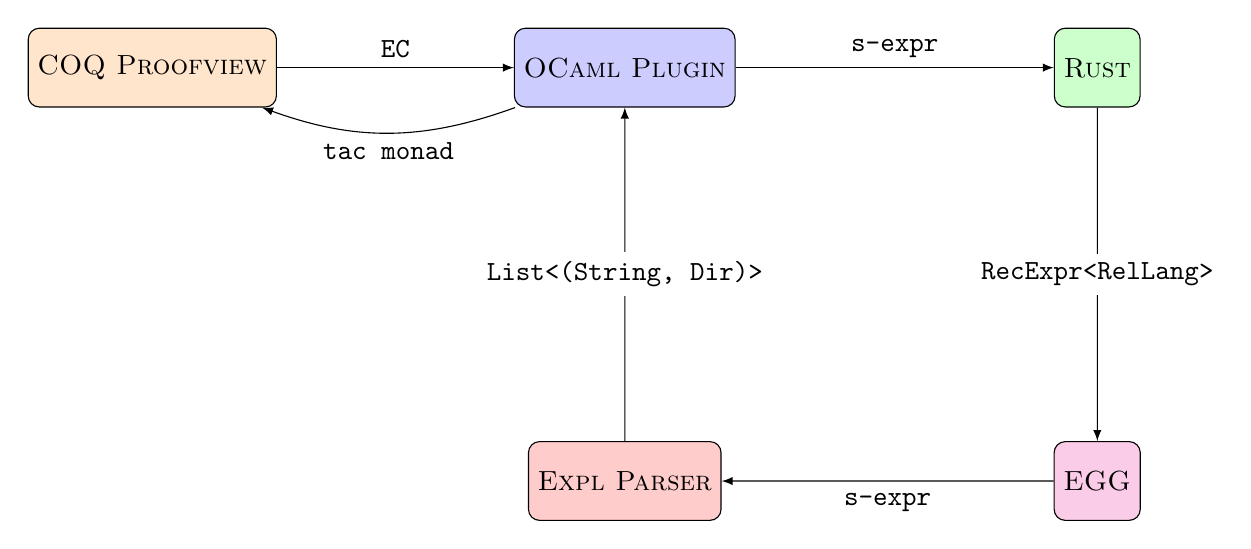
\begin{tikzpicture}[ampersand replacement=\&, scale=1.5]
        \node[rectangle, rounded corners, draw, fill=orange!20, minimum height=1cm] at (0,0) (CP) {\textsc{COQ Proofview}};
        \node[rectangle, rounded corners, draw, fill=blue!20, minimum height=1cm] at (4,0) (OP) {\textsc{OCaml Plugin}};	
        \node[rectangle, rounded corners, draw, fill=green!20, minimum height=1cm] at (8,0) (RUST) {\textsc{Rust}};	
        \node[rectangle, rounded corners, draw, fill=magenta!20, minimum height=1cm] at (8,-3.5) (EGG) {\textsc{EGG}};	
        \node[rectangle, rounded corners, draw, fill=red!20, minimum height=1cm] at (4,-3.5) (EP) {\textsc{Expl Parser}};	

        \draw [-latex] (CP) to node [above, sloped] (TextNode1) {\texttt{EC}} (OP);
        \draw [-latex] (OP) to node [above, sloped] (TextNode1) {\texttt{s-expr}} (RUST);
        \draw [-latex] (RUST) to node [fill=white] (TextNode1) {\texttt{RecExpr<RelLang>}} (EGG);
        \draw [-latex] (EGG) to node [below, sloped] (TextNode1) {\texttt{s-expr}} (EP);
        \draw [-latex] (EP) to node [fill=white] (TextNode1) {\texttt{List<(String, Dir)>}} (OP);
        \draw [-latex] (OP) to[bend left=20] node [below] (TextNode1) {\texttt{tac monad}} (CP);

    \end{tikzpicture}
    \caption{Components of the system}\label{fig:components}
\end{figure}

Data types over each arrow from Figure~\ref{fig:components} will be discussed in detail in the following chapter.  

\subsection{Vernacular Commands}
To extend Coq's grammar with a new tactic or command, one should write a \texttt{.mlg} file, where the tactic's syntax is defined. Consider an example: 

\vspace{0.5cm}
\begin{lstlisting}[language=ocaml_vernac, label=lst:mlg_example]
    DECLARE PLUGIN "coq-via-egg-plugin.plugin"

    VERNAC COMMAND EXTEND cegg_config CLASSIFIED AS QUERY
    | [ "Cegg" "config" reference(r) ] -> { ... } 
    END

    TACTIC EXTEND cegg_solve
    | [ "Cegg" "solve" ] -> { ... } (* Paring and interpretation rule *)
    END
\end{lstlisting}

In listing~\ref{lst:mlg_example}, we define a command called \texttt{cegg\_config} and a tactic called \texttt{cegg\_solve}. A command is marked as \texttt{QUERY}, meaning it is a \textit{pure} function. Otherwise it would have been marked as \texttt{SIDEFF}. 
\begin{definition}[Pure function]
    A pure function is a function where the return value is only determined by its input values, without observable side effects. 
\end{definition}
After the \texttt{|} symbol, we define the parsing rule and the the interpretation rule, separated by \texttt{->}. The parsing rule itself is a set of terminals that are matched against a string of tokens. The interpretation rule is a function that is called when the parsing rule is matched. More on the \texttt{.mlg} file format can be found in the Coq's plugin guide~\footnote{\href{https://github.com/coq/coq/blob/master/doc/plugin\_tutorial/tuto2/src/g\_tuto2.mlg}{https://github.com/coq/coq/blob/master/doc/plugin\_tutorial/tuto2/src/g\_tuto2.mlg}}.

\subsection{OCaml plugin}
When our tactic is called from inside the Coq proof, firstly, we need to extract the goal. Consider an example: 

\vspace{0.5cm}
\begin{lstlisting}[language=coq]
Lemma example (r : relation A) : 
    r^* ;; r^? (@\equiv@) r^*.
Proof.
    Cegg solve eq. 
\end{lstlisting}

When we enter the interactive proof process, we see the following proof state: 

\vspace{0.5cm}
\begin{lstlisting}[language=coq]
    A : Type 
    r : relation A
    ============================
    r^* ;; r^? (@\equiv@) r^*
\end{lstlisting}

Current hypothesises are located above the line and the conclusion of the goal --- below. To interact with Coq from OCaml, we use the Coq-Api\footnote{\href{https://coq.github.io/doc/V8.16.0/api/coq-core/index.html}{https://coq.github.io/doc/V8.16.0/api/coq-core/index.html}}, which provides a widest functionality. To extract that information about the goal in OCaml we first enter the Proofview monad.

\begin{definition}[Monad]
    Monads serve as a representation of computations. Consider a computation to be similar to a function that transforms an input to an output, but with an additional component. This component represents the effect that the function has as a consequence of being executed.
\end{definition}

In the following function \texttt{t} denotes the goal. \texttt{enter} applies the goal-dependent tactic, with \texttt{(t -> unit tactic)} type in each goal independently. 

\vspace{0.5cm}
\begin{lstlisting}[language=ocaml]
    val enter : (t -> unit tactic) -> unit tactic
\end{lstlisting}

Now we see that our tactic, all in all, should be a function that takes goal (\texttt{Proofview.Goal.t}) as input and return a tactic monad (\texttt{unit tactic}). When we have such a function, \texttt{enter} will apply it to each goal. 

Having a \texttt{gl {:} Proofview.Goal.t} as input, we need to split it into the conclusion, hypotheses and the environment, using functions \texttt{concl}, \texttt{hyps} and \texttt{env} respectively. The most import for us is the \texttt{concl}, which we will get. It has a \texttt{EConstr.constr}, which is the most important datatype in Coq, namely the kernel term. It is used to represent expressions, which are built using a set of constructors that correspond to the different types and operations. 

% TODO: Жидокато в конце написал, надо лучше
Our next task is to prepare the conclusion for the \texttt{egg} use. \texttt{Econstr.t} (similar to \texttt{Econstr.constr}) has a huge list of constructors, but we are not expecting to handle most of them. For example, constructors such as \texttt{Forall} or \texttt{LetIn} are not something we expect to see in a proposition about relations. From the limitations of what kind of rules we can pass to \texttt{egg} we can infer that we want to handle particular relations and various operations on them, i.e.\ applications of functions. Moreover, after analysing the Hahn library and the imm code base, we have decided to add some concrete relations as constants: An empty relation, denoted as \texttt{(fun\_ \_ => False)}, which means that for any two elements of the given set are related, and a full relation, denoted as \texttt{(fun \_ \_ => True)}. Thereby the constructors we are interested in are as follows: 

\vspace{0.5cm}
\begin{lstlisting}[language=ocaml]
    type Econstr.constr = 
        | App of 'constr * 'constr array
        | Var of Names.Id.t
        | Lambda of Names.Name.t Context.binder_annot * 'types * 'constr
        | Ind of Names.inductive * 'univs (* Inductive constructors, e.g. True or False *)
\end{lstlisting}

\texttt{Econstr.t} is parsed into a smaller type, which will be then transferred to \texttt{egg}. If unexpected constructors occur in the expression, exception is raised and a error is shown to the user. Data type is an s-expression over strings, with an addition of lambdas: 

\vspace{0.5cm}
\begin{lstlisting}[language=ocaml]
    type goal_s_expr =
        | Symbol of string
        | Application of string * goal_s_expr list
        | Lambda of goal_s_expr * goal_s_expr
\end{lstlisting}

Next step is to pass an object of type \texttt{goal\_s\_expr} to Rust for further processing. We use the \texttt{ocaml-rs}~\cite{OCaml_rust_ffi} Rust library to set up communication between OCaml and Rust. Similar type as \texttt{goal\_s\_expr} is defined in Rust: 

\vspace{0.5cm}
\begin{lstlisting}[language=rust, style=colouredRust]
    pub enum GoalSExpr {
        Symbol(String),
        Application(String, LinkedList<GoalSExpr>),
        Lambda(Box<GoalSExpr>, Box<GoalSExpr>),
    }
\end{lstlisting}

\subsection{Using Egg}



